\chapter{Binocular vision and Stereopsis}
\label{chap:BinocularVision}

Binocular Vision is a term used for the visual system of animals with two eyes \cite{how95}, and therefore, applies to human visual system as well. 
Possessing binocular vision not only lead to a better perception of depth
of the surrounding environment, but also help to better perform many visual tasks such as reading, object detection, interaction with surrounding objects such as grabbing and other manipulative 
tasks. However, the most significant advantage of possessing binocular vision is its influence on how the 3D environment, i.e. the depth of surrounding objects relative to each other, 
is perceived by the two eyes. This visual perception of depth in binocular vision is referred to as {\it Stereoscopic Vision}.
In the visual system, depth perception is a phenomenon that normally occurs though different types of cues and information existing in the surrounding environment. 
These pieces of information, known as {\it depth cues} in stereo vision, can be either monocular or binocular depth cues \cite{how95}.
To name a few instances of monocular depth cues, we can refer to motion parallax, lighting and shading, and apparent size. 
However, as previously mentioned, binocular cues which can only be perceived
by stereo vision, play a major role in the perception of depth. One of the most important binocular cues is {\it binocular disparity}, or {\it binocular parallax}. 
It should be noted that the effect of binocular parallax and motion parallax on depth perception are very similar to each other. 
In motion parallax, which is a monocular depth cue, the scene is viewed at different times by the observer moving from side to side, 
whereas in binocular parallax, the scene is viewed from slightly different viewpoints at
the same time by the two eyes, while the observer standing at a fixed position \cite{how95}. \textbf{FIGURE to show this}

\begin{figure}[!h]
\centering
\subcaptionbox{Motion Parallax}
[.4\linewidth]{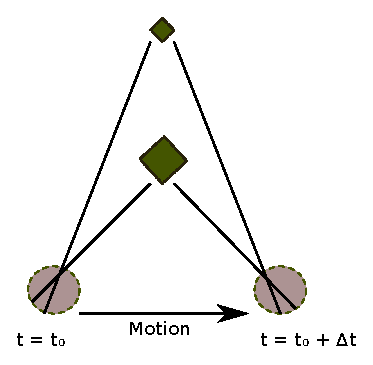
\includegraphics{Mparallax}}%
\subcaptionbox{Binocular Parallax}
[.4\linewidth]{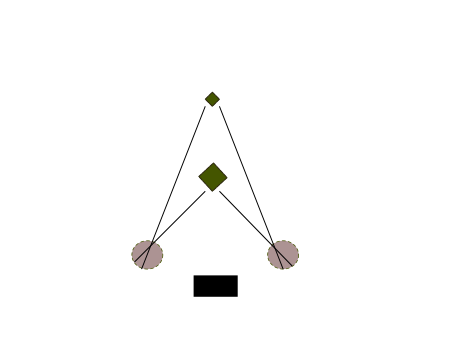
\includegraphics{Bparallax}}%
\caption{Motion parallax and binocular arallax difference}
\label{fig:parallax}
\end{figure}

%\begin{figure}[!h]
%\centering
%\begin{subfigure}[b]{7cm}            
%\frame{\includesvg[width=\textwidth]{Bparallax}}
%\caption{Interpolation for Data 1}
%\label{Fig:bp}
%\end{subfigure}
%
%\hspace{1cm}
%
%\begin{subfigure}[b]{7cm}
%\centering
%\frame{\includesvg[width=\textwidth]{Mparallax}}
%\caption{Interpolation for Data 2}
%\label{fig:mparallax}
%\end{subfigure}
%\caption{blah blah}\label{fig:bpmp}
%\end{figure}

Binocular disparity, which in fact arises from the spatial difference 
between the images of the same scene in the two eyes, provides a relative perception of depth from the surrounding environment. This perception is known as {\it binocular stereopsis} \cite{how95}. 
Another important binocular depth cue is the eyes {\it vergence}, which is the simultaneous movement of the pupils in opposite directions in order to obtain a single vision of an object with the
two eyes. When focusing on an object, the optical axes of the eyes intersect on the object of interest resulting in an angle called vergence angle. Unlike many animals, human visual system 
is capable of adjusting this angle based on the distance from the object.
In stereo vision, the locus of the points that yields a single vision in the visual system is known as the {\it horopter}, and any point located on the horopter is usually called a 
{\it fixation point} \cite{binr83,how95}.
An important property of an object on the horopter is that no spatial difference
exists between the images of the fixated object in the two eyes; i.e. the binocular disparity is zero \cite{how95}. 
Exploiting this property, the disparity of any other object in the scene can be estimated relative to the fixated object by inspecting two important factors: 
whether the object of interest is closer or further than the fixated object and then how much closer or further it is relative to the fixated object.
As a result, the binocular disparity provides a relative perception of depth of the surrounding environment.
In the geometry of stereopsis, the relative disparity between two objects is usually presented as angular disparity in radiant, or seconds of arc.

\section{Stereopsis Geometry and Angular Disparity}

In the following section, we will describe how the angular disparity can be calculated utilizing the geometry of stereopsis \cite{binr83}.

\begin{figure}[!h]
\centering
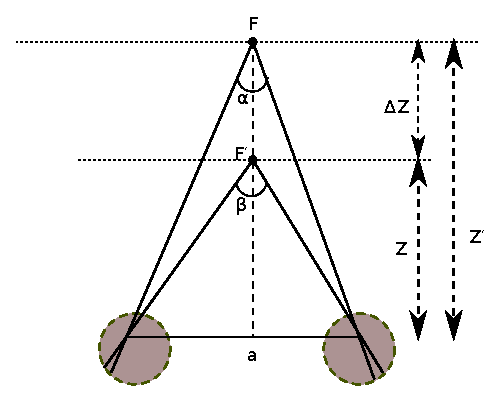
\includegraphics[width=0.5\textwidth]{binocular}
\caption{Binocular disparity}
\label{fig:stereopsis}
\end{figure} 

According to Figure \ref{fig:stereopsis}, we have:
\begin{align}
\theta = \beta - \alpha\\
\alpha = a/Z^{'}\\
\beta = a/Z\\
Z = Z^{'} + \Delta Z\\
\Rightarrow \theta = a/Z - a/Z^{'} = a/Z - a/(Z+\Delta Z) \\
\Rightarrow \theta = aZ+a\Delta Z-aZ/Z(Z+\Delta Z) = a\Delta Z/Z^{2} 
\end{align}

However, when $\Delta Z$ is very small compared to the values of $Z$, the term $\Delta Z$ in denominator can be neglected without significant loss of accuracy. This results in
an approximate formula as follows:

\begin{align}
\label{eq:stac}
\theta = a \Delta Z/Z^{2}
\end{align}

in which $a$ is the distance between the center of the pupils of the two eyes, which is known as interpupillary distance.
It should be noted that this formula estimates the angular disparity in radiant. In order to convert $\theta$ to arcseconds it should be multiplied by:

\begin{align}
180/\pi = 57.296\times360=206.265
\end{align}

Studies show that the visual system capability to distinguish two objects at different distances relative to each other is limited to certain thresholds \cite{binr83,how95}.
This threshold, which is defined as the minimum detectable depth between two 
objects at difference distances, is known as {\it stereoacuity} which varies in different visual systems \cite{binr83,how95}. According to different
experiments \cite{binr83}, the finest detectable angular disparity in human visual system is approximately 10-15 arcseconds. However, a more recent study on
stereoacuity in 60 subjects \cite{garn06} for different age groups, from 17 to 83 using standard stereotests, 
shows that the average stereoacuity for different age groups is as follows:

\begin{minipage}{\linewidth}
\begin{center}
\captionof{table}{Average stereoacuity for subjects of age 17 to 83}
\label{tab:stAcAge}
\begin{tabular}{ |c|c| }
\hline
\textbf{Age Range} & \textbf{Stereo Acuity (arcsecs)} \\ \hline
17-29 & 32 \\  \hline
30-49 & 33.75 \\ \hline
50-69 & 38.75 \\ \hline
70-83 & 112.5 \\ \hline
\end{tabular}
\end{center}
\end{minipage} \newline \newline

Furthermore, studies show that the average interpupillary distance in human is 64mm \cite{how95}. 
Using these values in equation \ref{eq:stac}, the threshold for minimum detectable relative depth 
between two objects can be estimated based on their distance from the observer. \newline 
Studying these concepts and related works in stereo vision, we have designed and implemented our evaluation framework based on standard
stereoacuity measurements mentioned in table \ref{tab:stAcAge}.
